\documentclass{amsart}
% 
\usepackage{graphicx}
\usepackage{picinpar}
\usepackage{caption}
\usepackage{float}
\usepackage[style=numeric, backend=biber]{biblatex}
\usepackage[yyyymmdd, hhmmss]{datetime}
\usepackage{xifthen}
% 
% 
\renewbibmacro{in:}{%
    \ifentrytype{article}{}{\printtext{\bibstring{in}\intitlepunct}}}
% 
% 
\newcommand{\closure}[1]{\mkern 1.5mu \overline{\mkern-1.5mu#1\mkern-1.5mu}\mkern 1.5mu}  % \var is too short and \overline is too long.  
% 
\newcommand{\closureit}[1]{\mkern 1.5mu \overline{\mkern-2.5mu#1\mkern-0.5mu}\mkern 1.5mu}  % \var is too short and \overline is too long.  
% 
% 
%\newcommand{\parallelsum}{\mathbin{\|}}
\newcommand{\parallelsum}{\mathbin{\!/\mkern-5mu/\!}}
% 
% 
\theoremstyle{plain}
\newtheorem{Theorem}{Theorem}
\newtheorem{TheoremCited}{Theorem}[section]
\newtheorem{Lemma}{Lemma}[section]
\newtheorem{Proposition}{Proposition}[section]
\newtheorem{Corollary}{Corollary}[section]
\newtheorem*{Theorem*}{Theorem}
\newtheorem*{Lemma*}{Lemma}
\newtheorem*{Proposition*}{Proposition}
\newtheorem*{Corollary*}{Corollary}
\newtheorem*{SinkNeighborhood*}{Theorem \ref{sink_neighborhood}}
\newtheorem*{MainTheorem*}{Theorem \ref{main_theorem}}
% 
\theoremstyle{definition}
\newtheorem{Definition}{Definition}[section]
\newtheorem*{Definition*}{Definition}
% 
\theoremstyle{remark}
\newtheorem{Remark}{Remark}[section]
\newtheorem*{Remark*}{Remark}
\newtheorem{Claim}{Claim}[section]
\newtheorem*{Claim*}{Claim}
% 
% 
% 
% 
\bibliography{flatdisk}
% 
\begin{document}
% 
\title{A GEODESIC-PRESERVING MAP OF A EUCLIDEAN CONE DISK IS AFFINE}
\author{QIANG GAO}
% 
\address{Department of Mathematics, Sun Yat-Sen University, 510275, Guangzhou, P. R. China}
\email{ gaoqiangks@outlook.com}
\thanks{The author is partially supported by NSFC, No: 11771456.  }
% 
% 
\begin{abstract}
    In this paper, we solve a rigidity problem on geodesic-preserving maps of the unit disk $\mathbb{D}$ into itself.  The unit disk $\mathbb{D}$ is equipped with a Euclidean cone metric which is induced by the lift of a holomorphic quadratic differential on a compact Riemann surface.  The main result is that an injective map of the disk into itself is an affine homeomorphism if it is geodesic-preserving.  
% 
\bigskip
% 
% 
\noindent AMS Mathematics Subject Classification (2010): 51F99; 30F45; 30F30; 
% 
\medskip
% 
\noindent Keywords: Holomorphic quadratic differential; geodesic-preserving; affine.  
\end{abstract}
% 
% 
\maketitle
% 
\section{Introduction}
% 
\noindent Let $\mathbb{R}^n$ be the n-dimensional Euclidean space.  A map $f: \mathbb{R}^n \mapsto \mathbb{R}^n$ is called geodesic-preserving if the image of a geodesic under $f$ is a geodesic.  It is a classical result in affine geometry that a geodesic-preserving map of the n-dimensional Euclidean space is affine.  Many mathematicians studied this kind of maps comprehensively.  For example, in conformal geometry, Beardon and Minda proved the following result.
%For example, the following theorem is due to Shulkin and Limbeek.  
%\begin{Theorem}[\cite{ShulkinLimbeek2017fundamental}]
%   Let $n \ge 2$ and  $\mathbb{T}^n=\mathbb{R}^n/\mathbb{Z}^n$ denote the standard n-torus.  Let $f : \mathbb{T}^n \mapsto \mathbb{T}^n$ be any bijection that maps lines to lines (as sets).  Then $f$ is affine.  
%\end{Theorem}
%In conformal geometry, Beardon and Minda proved the following 
\begin{Theorem}[\cite{BeardonMinda2002sphere}]
    A map $f : \hat{\mathbb{R}}^n \mapsto\hat{\mathbb{R}}^n $ is a M\"{o}bius transformation if and only if it is a locally sphere-preserving map.  
\end{Theorem}
% 
In hyperbolic geometry, the following result is due to Li and Wang.  
\begin{Theorem}[\cite{LiWangFundamental2016}]
    Suppose that $f : \mathbb{D}^n \mapsto \mathbb{D}^n $ is injective and maps any r-hyperplane into some r-hyperplane for some positive integer $r<n$.  Then it is an isometry or a composition of an isometry and an affine transformation under the Klein model if and only if $f$ is non-degenerate.  
\end{Theorem}
There are still many other generalizations.  For a more detailed list of such kind of rigidity results, we refer the reader to \cite{LiWangFundamental2016}.  In this paper, we study this problem in the unit disk with a Euclidean cone metric induced by the lift of a holomorphic quadratic differential on a compact Riemann surface.  The following is our main theorem:
\begin{Theorem} \label{main_theorem}
    Let $\phi$ be a holomorphic quadratic differential on a compact Riemann surface of genus $g \ge 2$ and $\tilde{\phi}$ be its lift to the unit disk $\mathbb{D}$.  Let $\mathbb{D}$ be equipped with the flat metric $|\tilde{\phi}|$.  Suppose that $f:\mathbb{D} \mapsto \mathbb{D}$ is injective and geodesic-preserving. Then $f$ is affine.  
\end{Theorem}
% 
% 
% 
\subsection*{Acknowledgement}
I would like to thank my advisor Lixin Liu for his careful reading of this manuscript and many useful suggestions, and I would like to thank Huiping Pan for useful conversations.  
% 
% 
\section{Background}
In this section, we recall some basic knowledge about holomorphic quadratic differentials and the related geometry.  
\subsection{The local geometry of quadratic differentials}
Given any holomorphic quadratic differential $\phi$ on a Riemann surface $X$, at every regular point $p\in X$, there exists a local coordinate $z$ on a sufficiently small neighborhood $U$ of $p$ such that $\phi=dz^2$ on $U$.  The coordinate $z$ is given by the integral $z(y)=\int^y_p\sqrt{\phi}$.  At every singular point $q$, there exists a local coordinate $z$ in a small neighborhood $V$ such that $\phi=z^kdz^2$ in $V$, where $k$ is the order of $\phi$ at $q$.  These are called the natural coordinates of holomorphic quadratic differentials.  For a detailed introduction, we refer the reader to \cite{Strebel84}.  Every holomorphic quadratic differential induces a metric that is singular at zeroes.  The local behavior of this metric in a neighborhood of a regular point is exactly Euclidean.  In a small neighborhood of a singular point of order $k$, this metric is obtained by patching together $k+2$ Euclidean half-spaces, as shown in the following picture.  
% 
\begin{figure}[h]
    \centering
    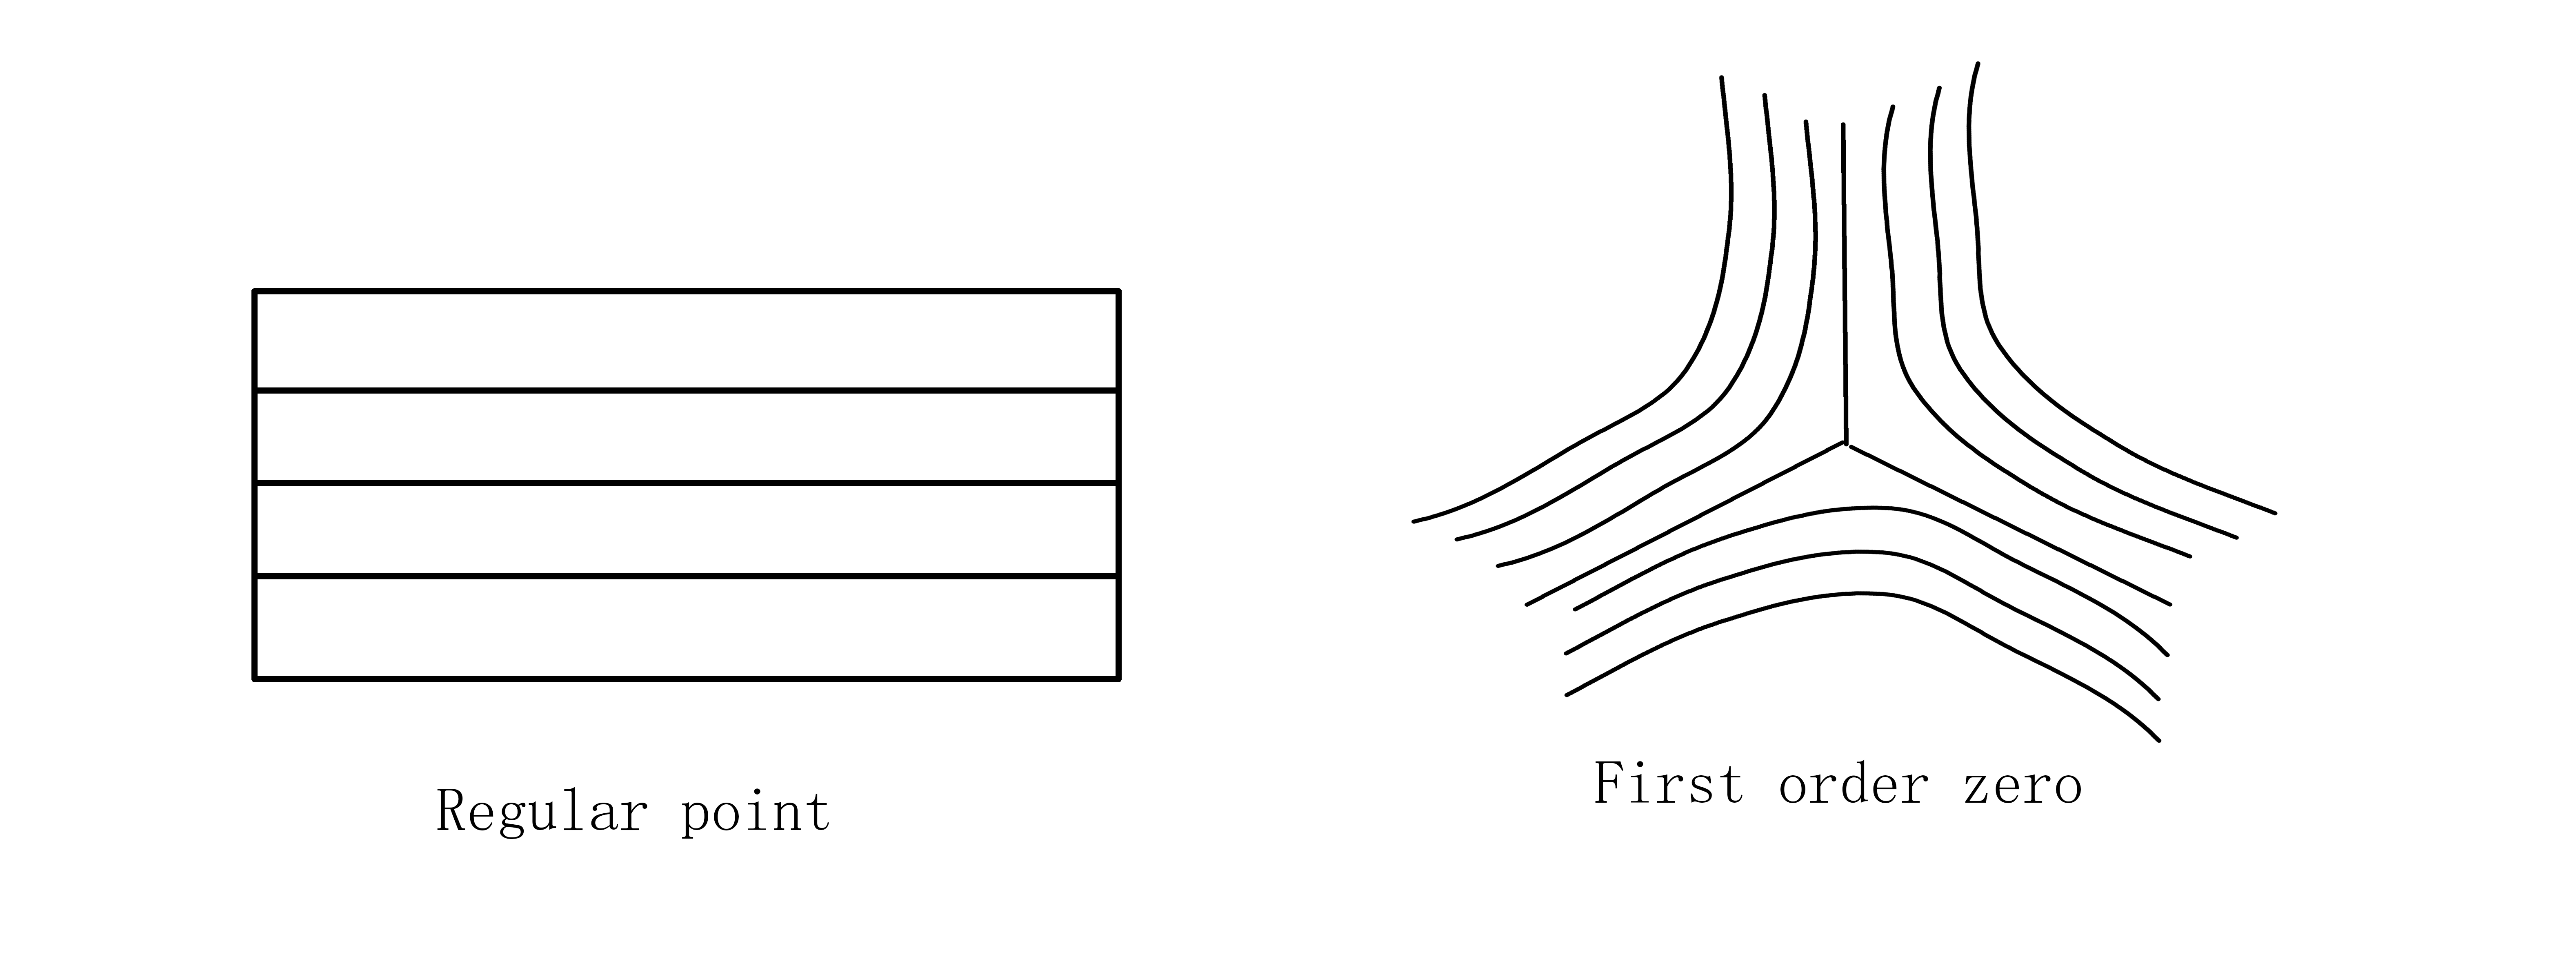
\includegraphics[scale=0.25]{critical_point.png}
    \caption{The local geometry of a holomorphic quadratic differential}
    \label{critical_point}
\end{figure}
% 
A $\theta$-trajectory of $\phi$ is defined to be the maximal extension of 
\begin{equation*}
\{z\in \mathbb{D}: arg\phi(z)=\theta \}.
\end{equation*}
% 
A geodesic segment is an isometric embedding of an interval $[a, b]$ into $\mathbb{D}$.  It is made up of a sequence of trajectories.  It's a classical result that two adjacent geodesic segments make up a new one if and only if the two angles they make are both greater than or equal to $\pi$.  A geodesic is said to be non-singular if it doesn't contain any singular point.  We always parameterize a geodesic (geodesic ray or geodesic segment) by length parameter and the choice of the base point should be clear from the context. \par 
% 
% 
We make some conventions for terms and notations.  We reserve the term geodesic to mean that it is of infinite length in both directions, and when we speak of a geodesic ray, we mean it is finite in one direction and infinite in the other.  The two endpoints of a geodesic $\gamma$ are denoted by $\gamma(+\infty)$ and $\gamma(-\infty)$ respectively.  The endpoint on the boundary of a geodesic ray $\alpha$ is denoted by $\alpha(+\infty)$.  The endpoints of a geodesic or geodesic ray are well defined by Theorem \ref{marden_strebel} below.
% 
\begin{Remark*}
We follow the convention that at any singular point $p$ of order $k$, the cone angle at $p$ is defined to be $(k+2)\pi$.  Other authors may use the intrinsic conformal angle which differs from ours by a factor $\frac{2}{k+2}$. \par
\end{Remark*}
\subsection{The large-scale geometry of quadratic differentials}
\subsection*{}
Teichm\"uller's lemma dominates the large-scale behavior of quadratic differentials.
\begin{Theorem}[Teichm\"uller's lemma] \label{teichmuller_lemma}
    Let G be the interior of a simple closed $\phi$-polygon $\Lambda$ with sides $\lambda_i$ and interior angles $\theta_j$ at its vertices.  The quadratic differential $\phi$ is supposed to be holomorphic in $\closureit{G}$ (the only points on $\Lambda$ which can be critical are the vertices).  The zeroes of $\phi$ in $G$ are denoted by $z_i$ with $n_i$ their orders.  Then we have
    \begin{equation*}
    \sum_j(\pi-\theta_j)=2\pi+\sum_in_i\pi, 
    \end{equation*}
    where $n_i$ ranges over all zeroes of $\phi$ in $G$.  
\end{Theorem}
The following results are crucial for our proof.  
\begin{Theorem}[\cite{MardenStrebel}] \label{marden_strebel}
    Let $\mathbb{D}$ be equipped with the metric $|\tilde{\phi}|$.  Then the following results hold:
    \begin{enumerate}
\item Any geodesic ray has a well-defined endpoint on $\partial \mathbb{D}$.
\item If $\gamma_1, \gamma_2$ are two geodesic rays emanating from a common origin O, then their endpoints are different.  
        \item If two geodesics $\gamma_1, \gamma_2$ share the same pair of endpoints on $\partial \mathbb{D}$, then they bound a Euclidean strip and the projection of $\gamma_1, \gamma_2$ are parallel simple loops.  
    \end{enumerate}
\end{Theorem}
% 
The large-scale geometry of $|\tilde{\phi}|$ behaves more like hyperbolic space despite that its local geometry is just Euclidean.  
% 
\begin{Definition}
    Two metric spaces $(X_1,d_1)$ and $(X_2,d_2)$ are called quasi-isometric if there exists a map $f$ between $X_1$ and $X_2$ satisfying: there exist constants $\lambda \ge 1, \epsilon > 0$ and $K\ge 0$ such that for any $x, y \in X_1$, 
    \begin{equation*}
    \frac{1}{\lambda}d_1(x, y) - \epsilon \le d_2(f(x), f(y)) \le \lambda d_1(x, y) + \epsilon ,
    \end{equation*}
    and every point of $X_2$ lies within a distance of $K$ of the image $f(X_1)$.  
\end{Definition}
Actually, since the fundamental group of a compact Riemann surface acts properly discontinuously and cocompactly on the unit disk $\mathbb{D}$, we can apply the classical \v{S}varc-Milnor lemma:
\begin{Corollary}
    The unit disk $\mathbb{D}$, when equipped with the metric induced by the lift of a holomorphic quadratic differential on a Riemann compact surface, is quasi-isometric to the hyperbolic space $\mathbb{D}_H$.  
\end{Corollary}
% 
The following is an immediate corollary  of the above result which plays an important role in our proof:
\begin{Corollary}
    There exists a constant K depending only on $\phi$ such that every geodesic $\gamma$ in the $|\tilde{\phi}|$ metric is in a K-neighborhood of the hyperbolic geodesic connecting $\gamma(+\infty)$ and $\gamma(-\infty)$.  
\end{Corollary}
% 
In the proof of surjectivity of $f$, we make use of a homeomorphism between the boundary $\partial \mathbb{D}$ and the space of geodesic rays emanating from a fixed point.  Fix any point $O\in \mathbb{D}$, if we equip the set of all geodesic rays $\mathcal{G}(O)$ emanating from $O$ with the compact-open topology, then the boundary of the unit disk $\partial \mathbb{D}$ can be naturally identified $\mathcal{G}(O)$.  Define a map $g : \mathcal{G}(O) \mapsto \partial \mathbb{D}$ in the following way: for any $\gamma \in \mathcal{G(O)}$, let $g(\gamma)=\gamma(+\infty)$.  Then
\begin{Theorem}
    The map $g$ is a homeomorphism.  
\end{Theorem}
For a detailed introduction of the above results, one can see \cite[Chapter D.3]{bridsonhaefliger2013metric} and \cite[Chapter 10]{Papadopoulos2014Metric}
% 
\section{Proof of the main result}
% 
% 
\noindent From now on, we always equip $\mathbb{D}$ with the metric $|\tilde{\phi}|$ unless otherwise stated.  When we speak of the map $f$, we mean the one defined in Theorem \ref{main_theorem}.
% 
\begin{Definition}
    A map of $\mathbb{D}$ into itself is called geodesic-preserving if the image of a geodesic is a geodesic.  
\end{Definition}
\begin{Definition}
    A geodesic chain is a finite sequence of geodesics $\{\gamma_k\}_{1\le k\le n}$ such that $\gamma_k\cap \gamma_{k+1} \ne \emptyset$ for $1 \le k<n$.  Two disjoint geodesics $\alpha, \beta$ are said to be connected by a geodesic chain $\Gamma$ if $\Gamma \cap \alpha \ne \emptyset$ and $\Gamma \cap \beta \ne \emptyset$.  
\end{Definition}
%\begin{MainTheorem*}
%   Let $\phi$ be a holomorphic quadratic differential on a compact Riemann surface of genus $g \ge 2$ and $\tilde{\phi}$ be its lift to the unit disk $\mathbb{D}$.  Let $\mathbb{D}$ be equipped with the flat metric $|\tilde{\phi}|$.  Suppose that $f:\mathbb{D} \mapsto \mathbb{D}$ is injective and geodesic-preserving. Then $f$ is affine.  
%\end{MainTheorem*}
% 
% 
\subsection{The map f is continuous on geodesics}
% 
\begin{Proposition} \label{lemma-endpoints-are-different}
    Suppose that $\gamma$ is a geodesic, and $p, q\in \gamma$.  Suppose that $\alpha, \beta$ are two geodesic rays emanating from $p, q$ respectively and lying on the same side of $\gamma$.  The two angles formed by $\overline{pq}$ and $ \alpha$ , $\overline{qp}$ and $\beta$ are denoted by $\angle P $ and $\angle Q$ respectively, as shown in Figure \ref{figure-endpoints-are-different}.  If $\angle P + \angle Q > \pi$, then the endpoints of $\alpha$ and $\beta$ are different.  
\end{Proposition}
% 
\begin{figure}[H]
\centering
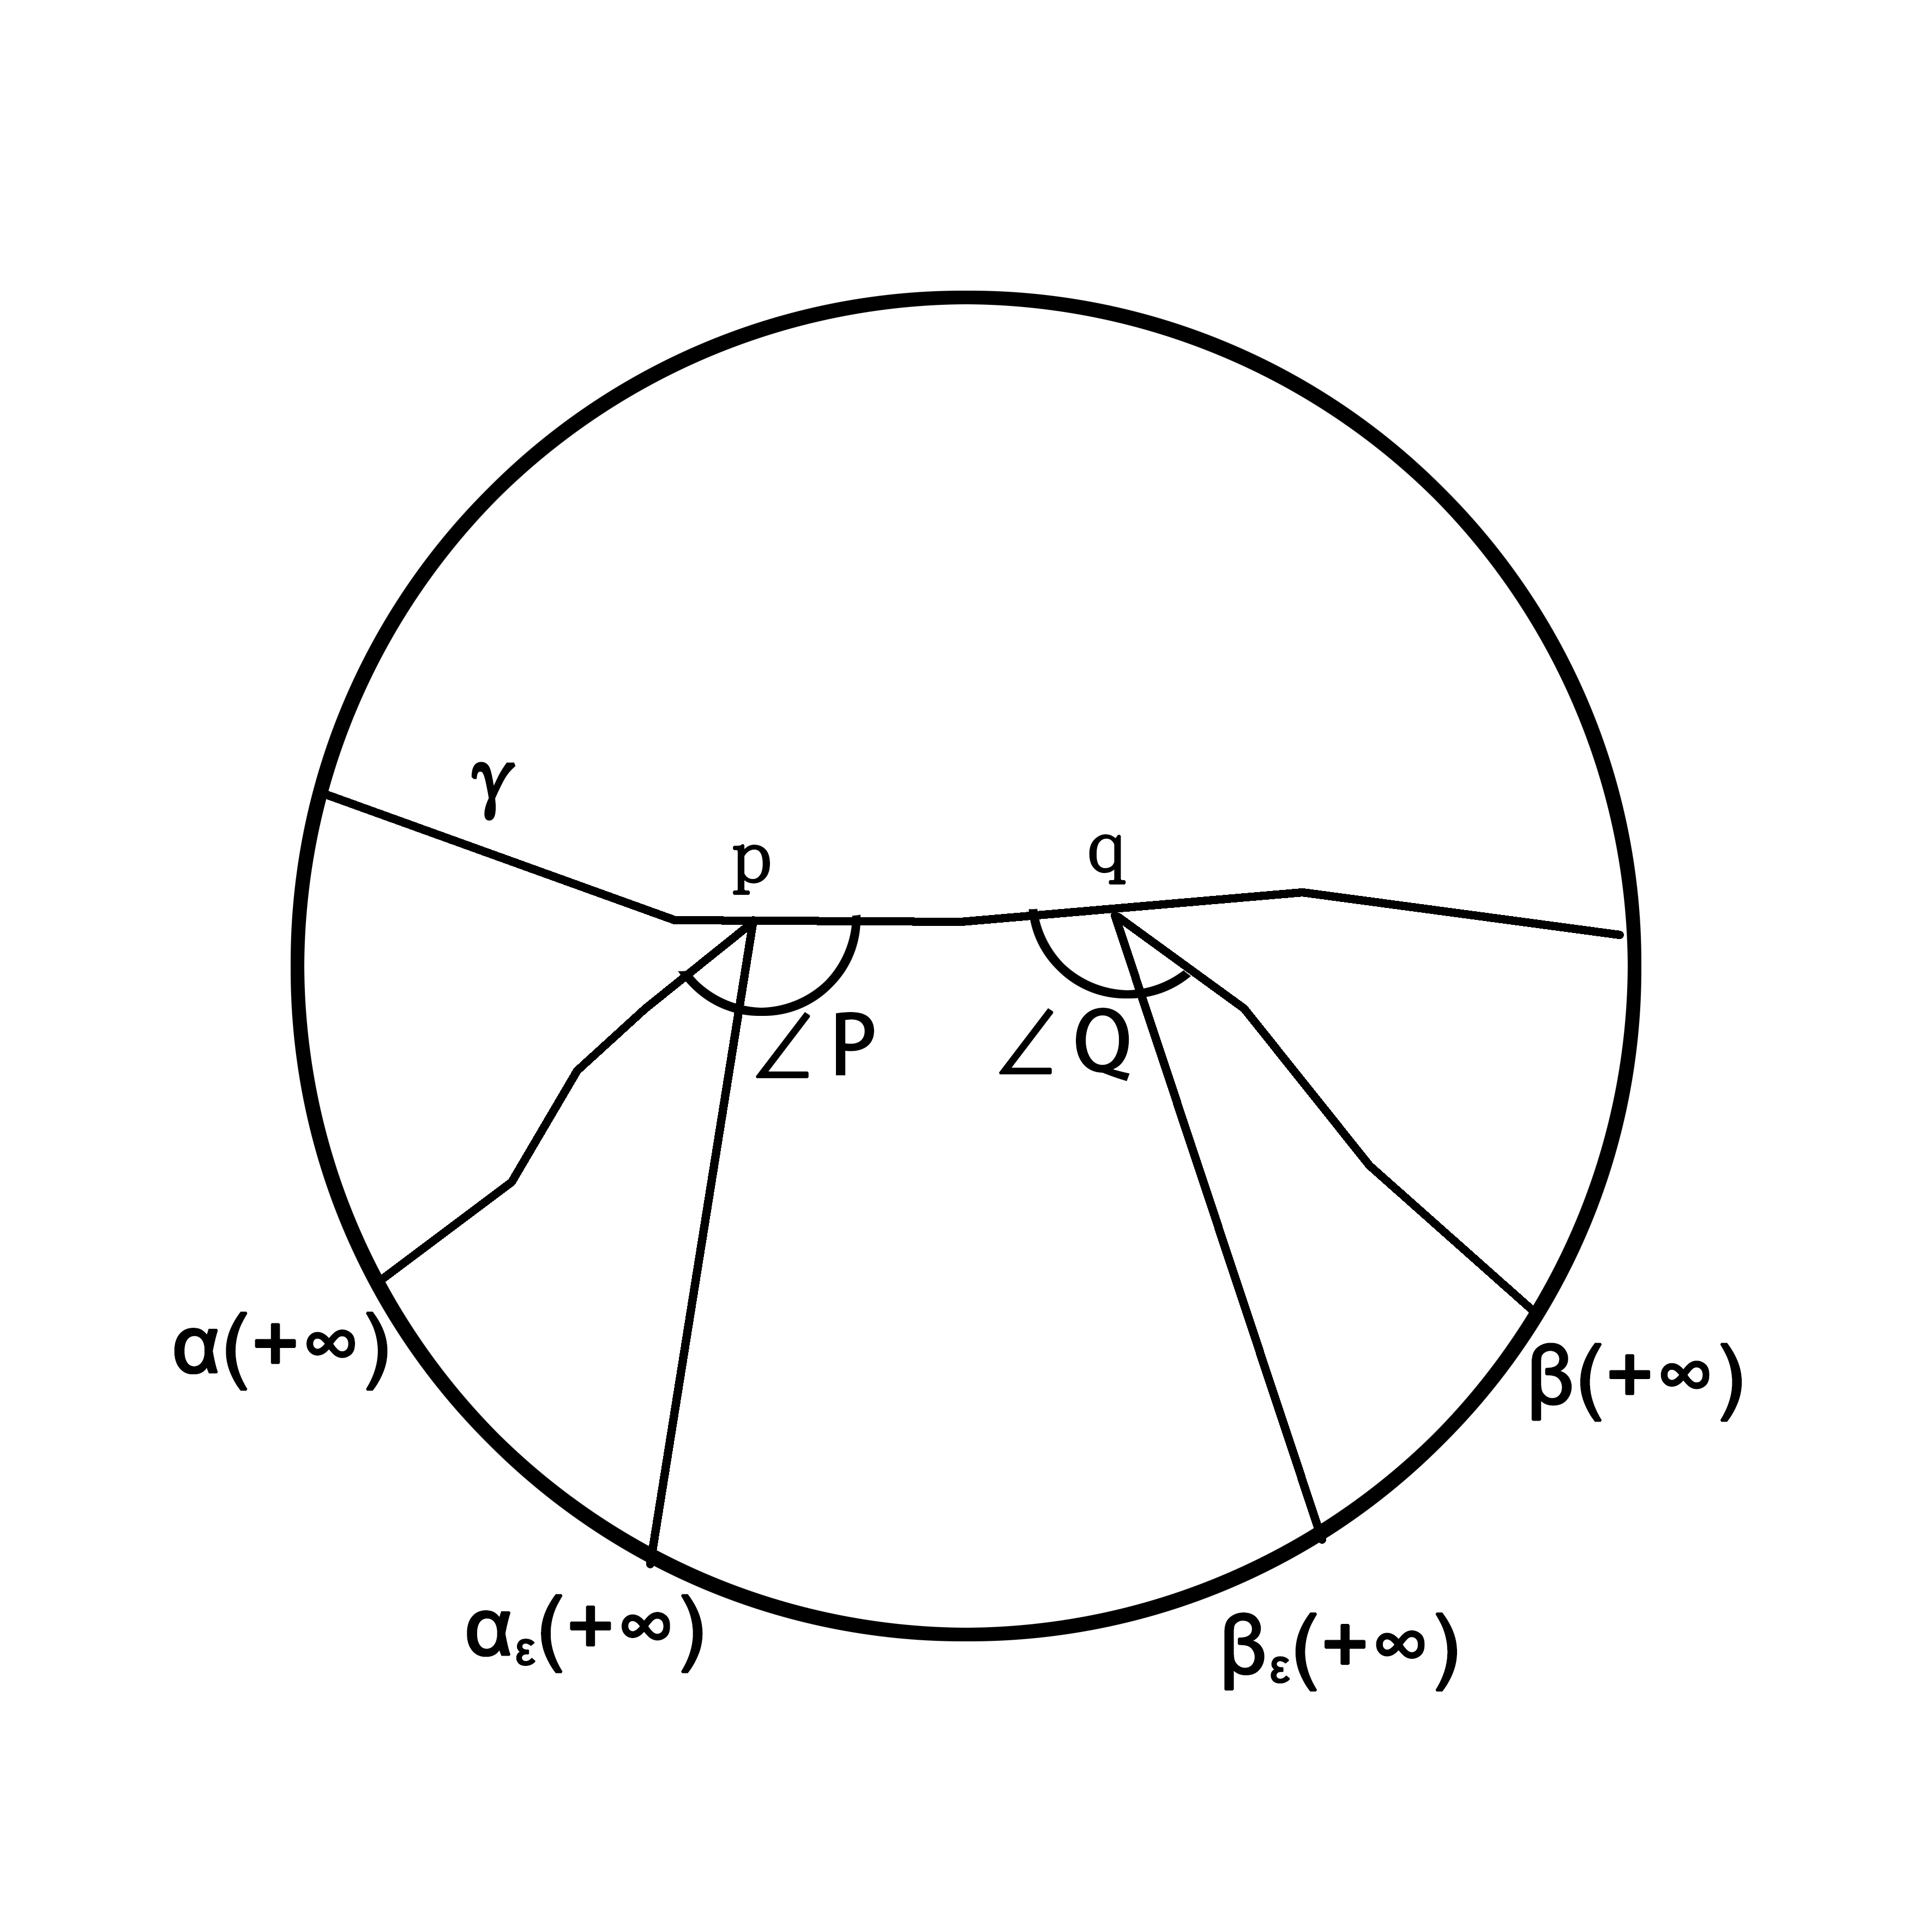
\includegraphics[scale=0.25]{divergence.png}
\caption{Two rays with different endpoints}
\label{figure-endpoints-are-different}
\end{figure}
\begin{proof}
    By Teichm\"uller's lemma, the two rays $\alpha$ and $\beta$ are disjoint.  Without loss of generality, we can assume that $\alpha$ is on the left side of $\beta$.  Take a geodesic ray $\alpha_{\epsilon}$ emanating from $p$ and on the right of $\alpha$ such that the angle formed by $\alpha_\epsilon$ and $\alpha$ is smaller than $\epsilon$.  By Theorem \ref{marden_strebel}, its endpoint is different from $\alpha(+\infty)$.  In the same way, we get a geodesic ray $\beta_\epsilon$ on the left of $\beta$.  Taking $\epsilon$ sufficiently small, we can make sure that $\alpha_\epsilon$ and $\beta_\epsilon$ are disjoint.  Therefore, the two endpoints $\alpha(+\infty)$ and $\beta(+\infty)$ are separated by $\alpha_\epsilon(+\infty)$  and $\beta_\epsilon(+\infty)$.  Obviously, they are different.  
\end{proof}
% 
The following lemma is the core of our proof.
% 
\begin{Lemma}\label{order-preserving}
    The restriction of $f$ to a geodesic $\gamma$ --- $f|_\gamma$ is order-preserving.  
\end{Lemma}
We first prove that if $A, B, C \in \gamma$ and $B$ is in the middle of $A$ and $C$, then $f(B)$ is also in the middle of $f(A)$ and $f(C)$.  A map $g: \mathbb{R} \mapsto \mathbb{R}$ satisfying this condition is said to have the middle-point-preserving property.  
% 
% 
\begin{Proposition} 
    There exist three geodesics $\gamma_A, \gamma_B$ and $\gamma_C$ satisfying the following conditions:
    \begin{enumerate}
        \item These three geodesics are pairwise disjoint.
        \item $\gamma_A(0)=A, \gamma_B(0)=B$ and $\gamma_C(0)=C$. The geodesic $\gamma_A$ has the property that the two subrays $\gamma_A(0, +\infty)$ and $\gamma_A(0, -\infty)$ lie on different sides of $\gamma$, and so do $\gamma_B$ and $\gamma_C$.  
        \item $\gamma_A(+\infty), \gamma_B(+\infty)$ and $\gamma_C(+\infty)$ lie on the same side of $\gamma$.
        \item $\gamma_A(+\infty), \gamma_B(+\infty), \gamma_C(+\infty)$ and the two endpoints of $\gamma$ are pairwise different.  
    \end{enumerate}
\end{Proposition}
% 
% 
\begin{figure}[h]
    \centering
    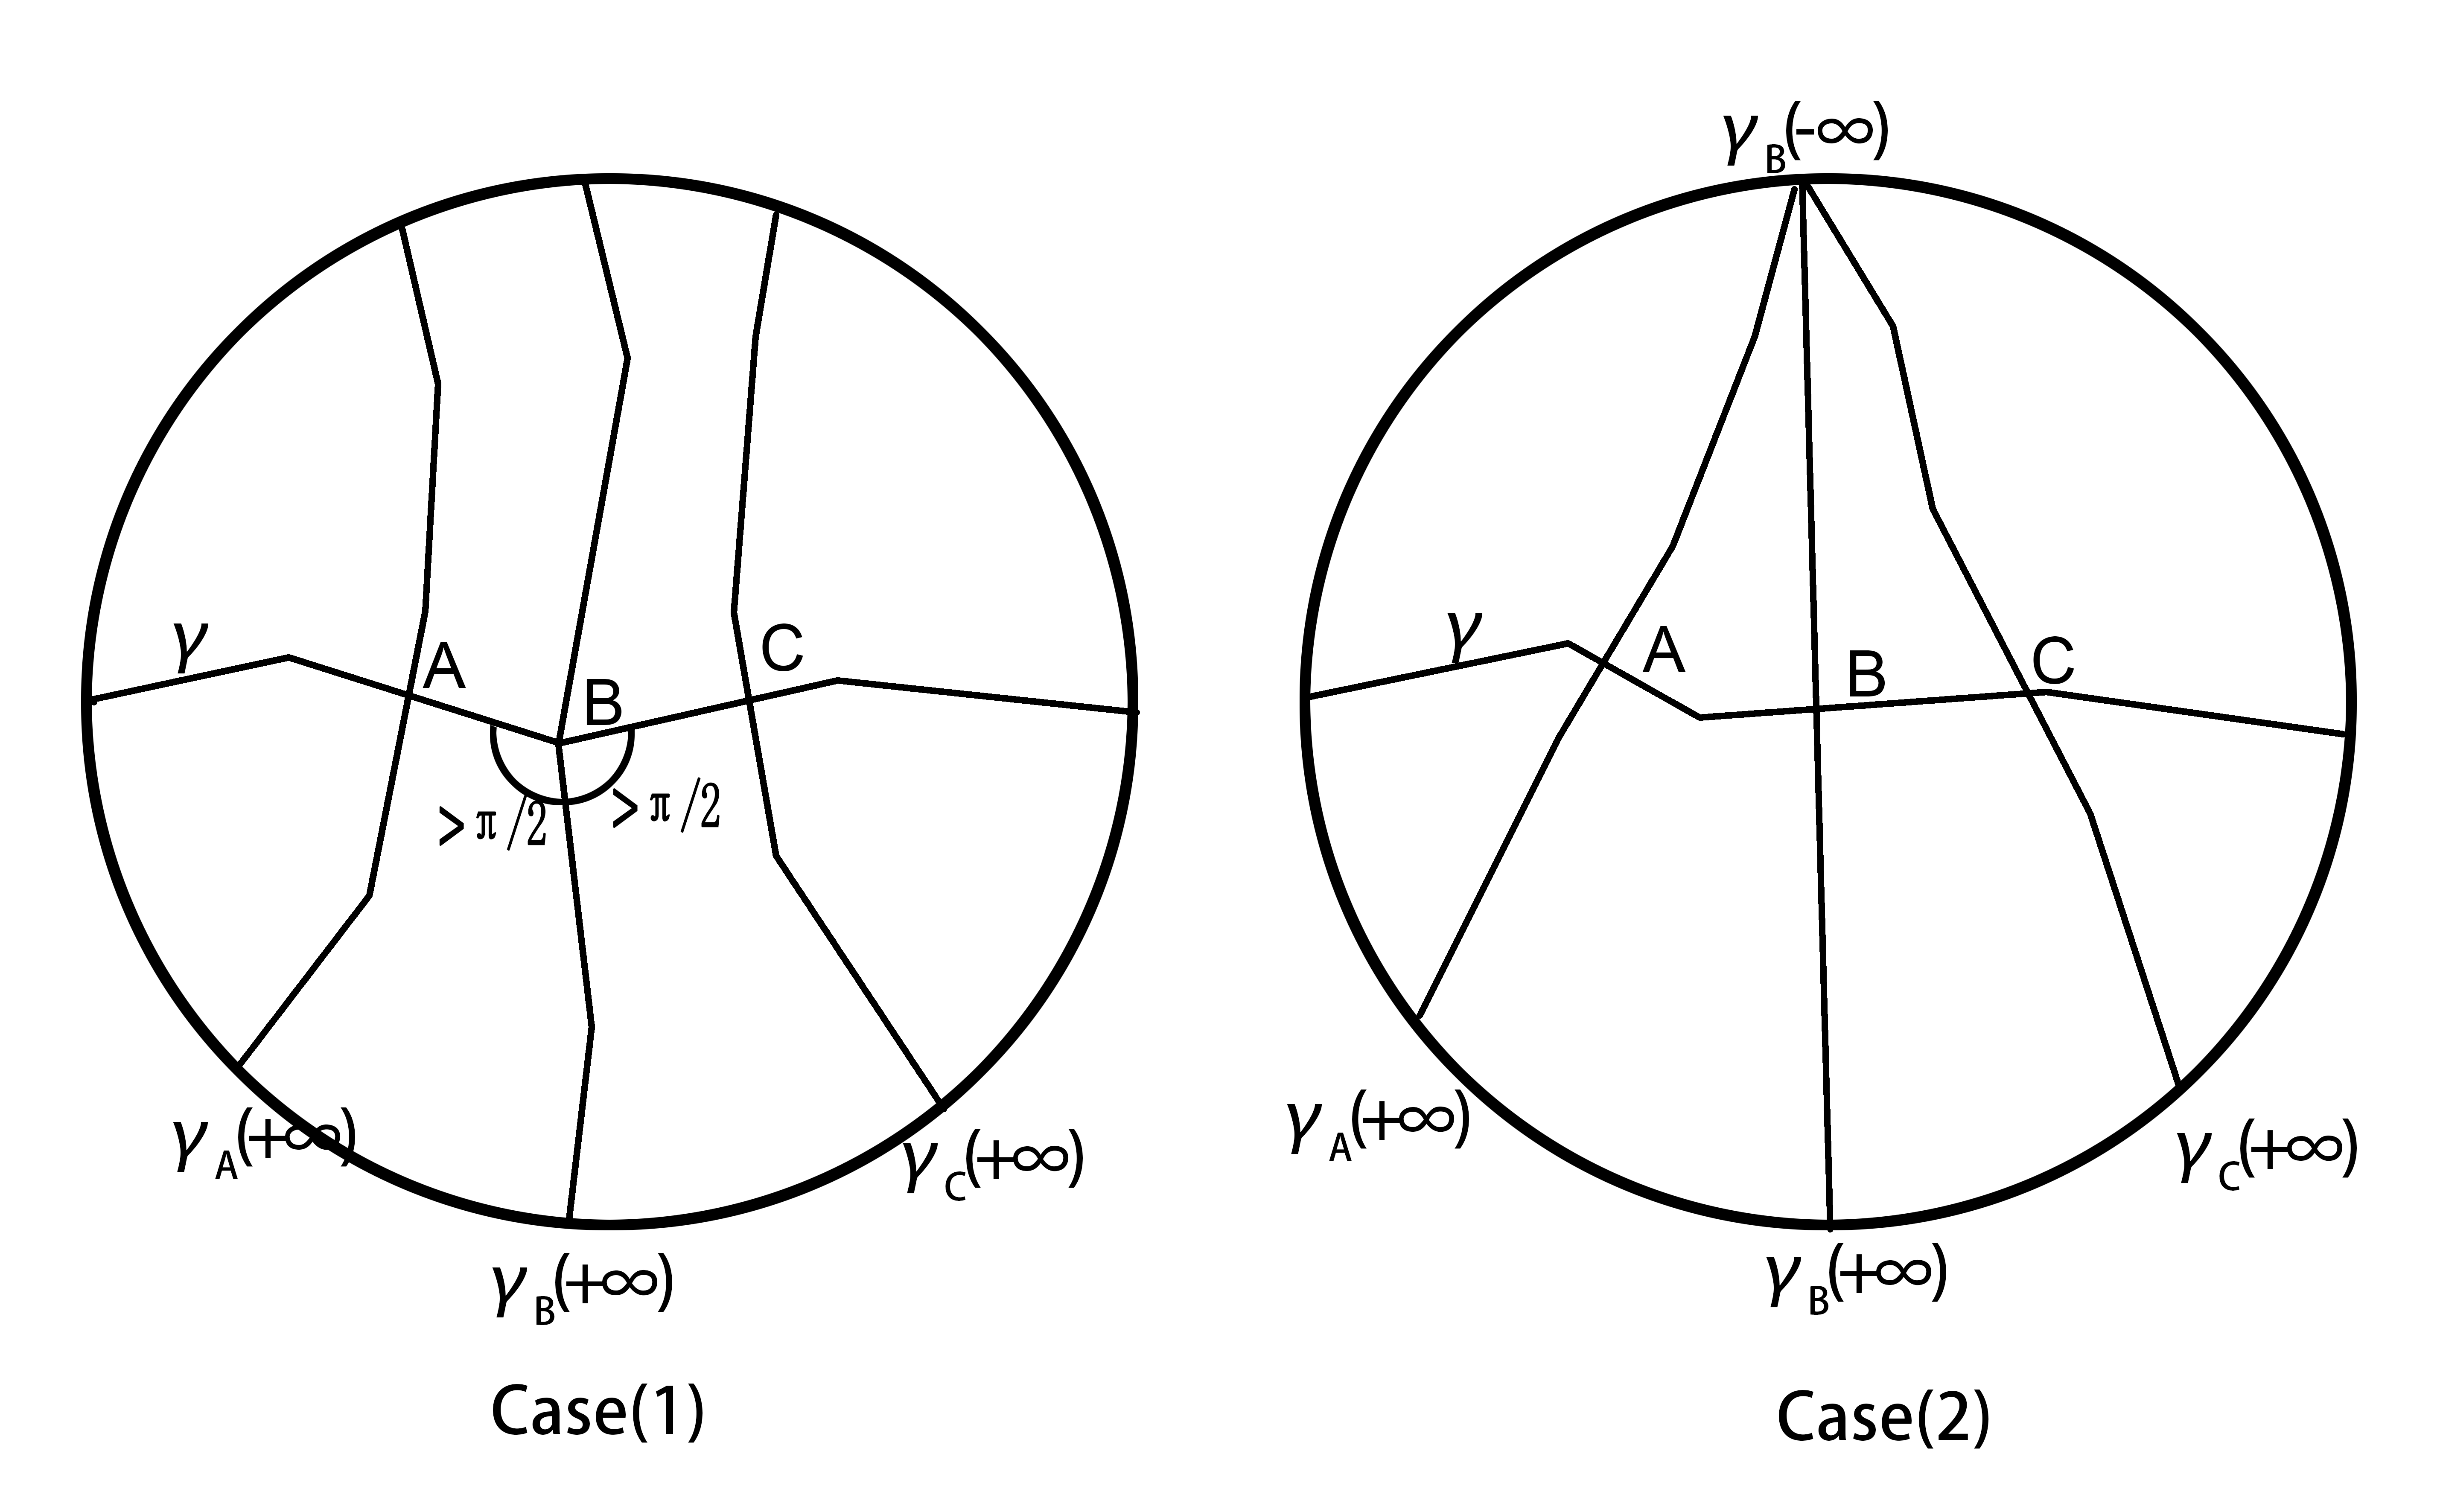
\includegraphics[scale=0.25]{three_geodesics.png}
    \caption{Three geodesics with different endpoints}
    \label{three-geodesics}
\end{figure}
% 
% 
\begin{proof}
    Since $\gamma$ is a geodesic, the two angles at $B$ formed by $\gamma$ are all greater than or equal to $\pi$.  
%     
    If $B$ is a singular point, extend the angular bisector of each angle formed by $\gamma$ at $B$ to the boundary.  Obviously, the composition of these two angular bisectors is geodesic which we denote by $\gamma_B$.  We can assume $\gamma_B(0)=B$.  Suppose the angle at $B$ formed by $\gamma$ on its bottom side is strictly greater than $\pi$, and the ray $\gamma_B(0, +\infty)$ lies on this side.  We construct $\gamma_A$ at $A$ and $\gamma_C$ at $C$ in the same way.  Then by Proposition \ref{lemma-endpoints-are-different}, the three geodesics $\gamma_A, \gamma_B$ and $\gamma_C$ are pairwise disjoint and their endpoints on the bottom side of $\gamma$ are all different.  See Figure \ref{three-geodesics} case(1).  
%     
    If $B$ is a normal point, consider the family of geodesics through $B$.  Any two of them intersect at a single point.  Since there are only countably many periodic directions and countably many singular points, almost every geodesic in this family is non-singular and non-periodic.  Choose a non-singular and non-periodic geodesic from this family, and denote it by $\gamma_B$.  Take the geodesic ray connecting $\gamma_B(-\infty)$ and $A$. Make it cross $\gamma$ and tend to the boundary.  We get a geodesic passing through $A$ and denote it by $\gamma_A$.  Similarly we get $\gamma_C$.  By Theorem \ref{marden_strebel}, these three geodesics are pairwise disjoint and their endpoints $\gamma_A(+\infty), \gamma(+\infty)$ and $\gamma_C(+\infty)$ are all different.  See Figure \ref{three-geodesics} case(2).  
\end{proof}
The two endpoints of $\gamma$ divide the boundary into two parts.  From now on, we'll work in the part which  $\gamma_A(+\infty), \gamma_B(+\infty)$ and $\gamma_C(+\infty)$ lie on.  In addition, we assume that $\gamma_A(+\infty), \gamma_B(+\infty)$ and $\gamma_C(+\infty)$ are in counter-clockwise order.  
\begin{Proposition}
    There are two geodesic chains $\Gamma_\alpha=\{\alpha_1, .  .  \alpha_n\}$ and $\Gamma_\beta=\{\beta_1, .  .  \beta_m\}$ satisfying the following conditions:
    \begin{enumerate}
        \item $\Gamma_\alpha \cap \gamma_A \ne \emptyset, \Gamma_\alpha \cap \gamma_B \ne \emptyset$ and $\Gamma_\alpha \cap \gamma_C = \emptyset $.
        \item $\Gamma_\beta \cap \gamma_B \ne \emptyset, \Gamma_\beta \cap \gamma_C \ne \emptyset$ and $\Gamma_\beta \cap \gamma_A = \emptyset $.
        \item $\Gamma_\alpha \cap \gamma = \emptyset, \Gamma_\beta \cap \gamma = \emptyset$.
        \item $\Gamma_\alpha \cap \Gamma_\beta \ne \emptyset$.
    \end{enumerate}  
\end{Proposition}
\begin{figure}[h]
    \centering
    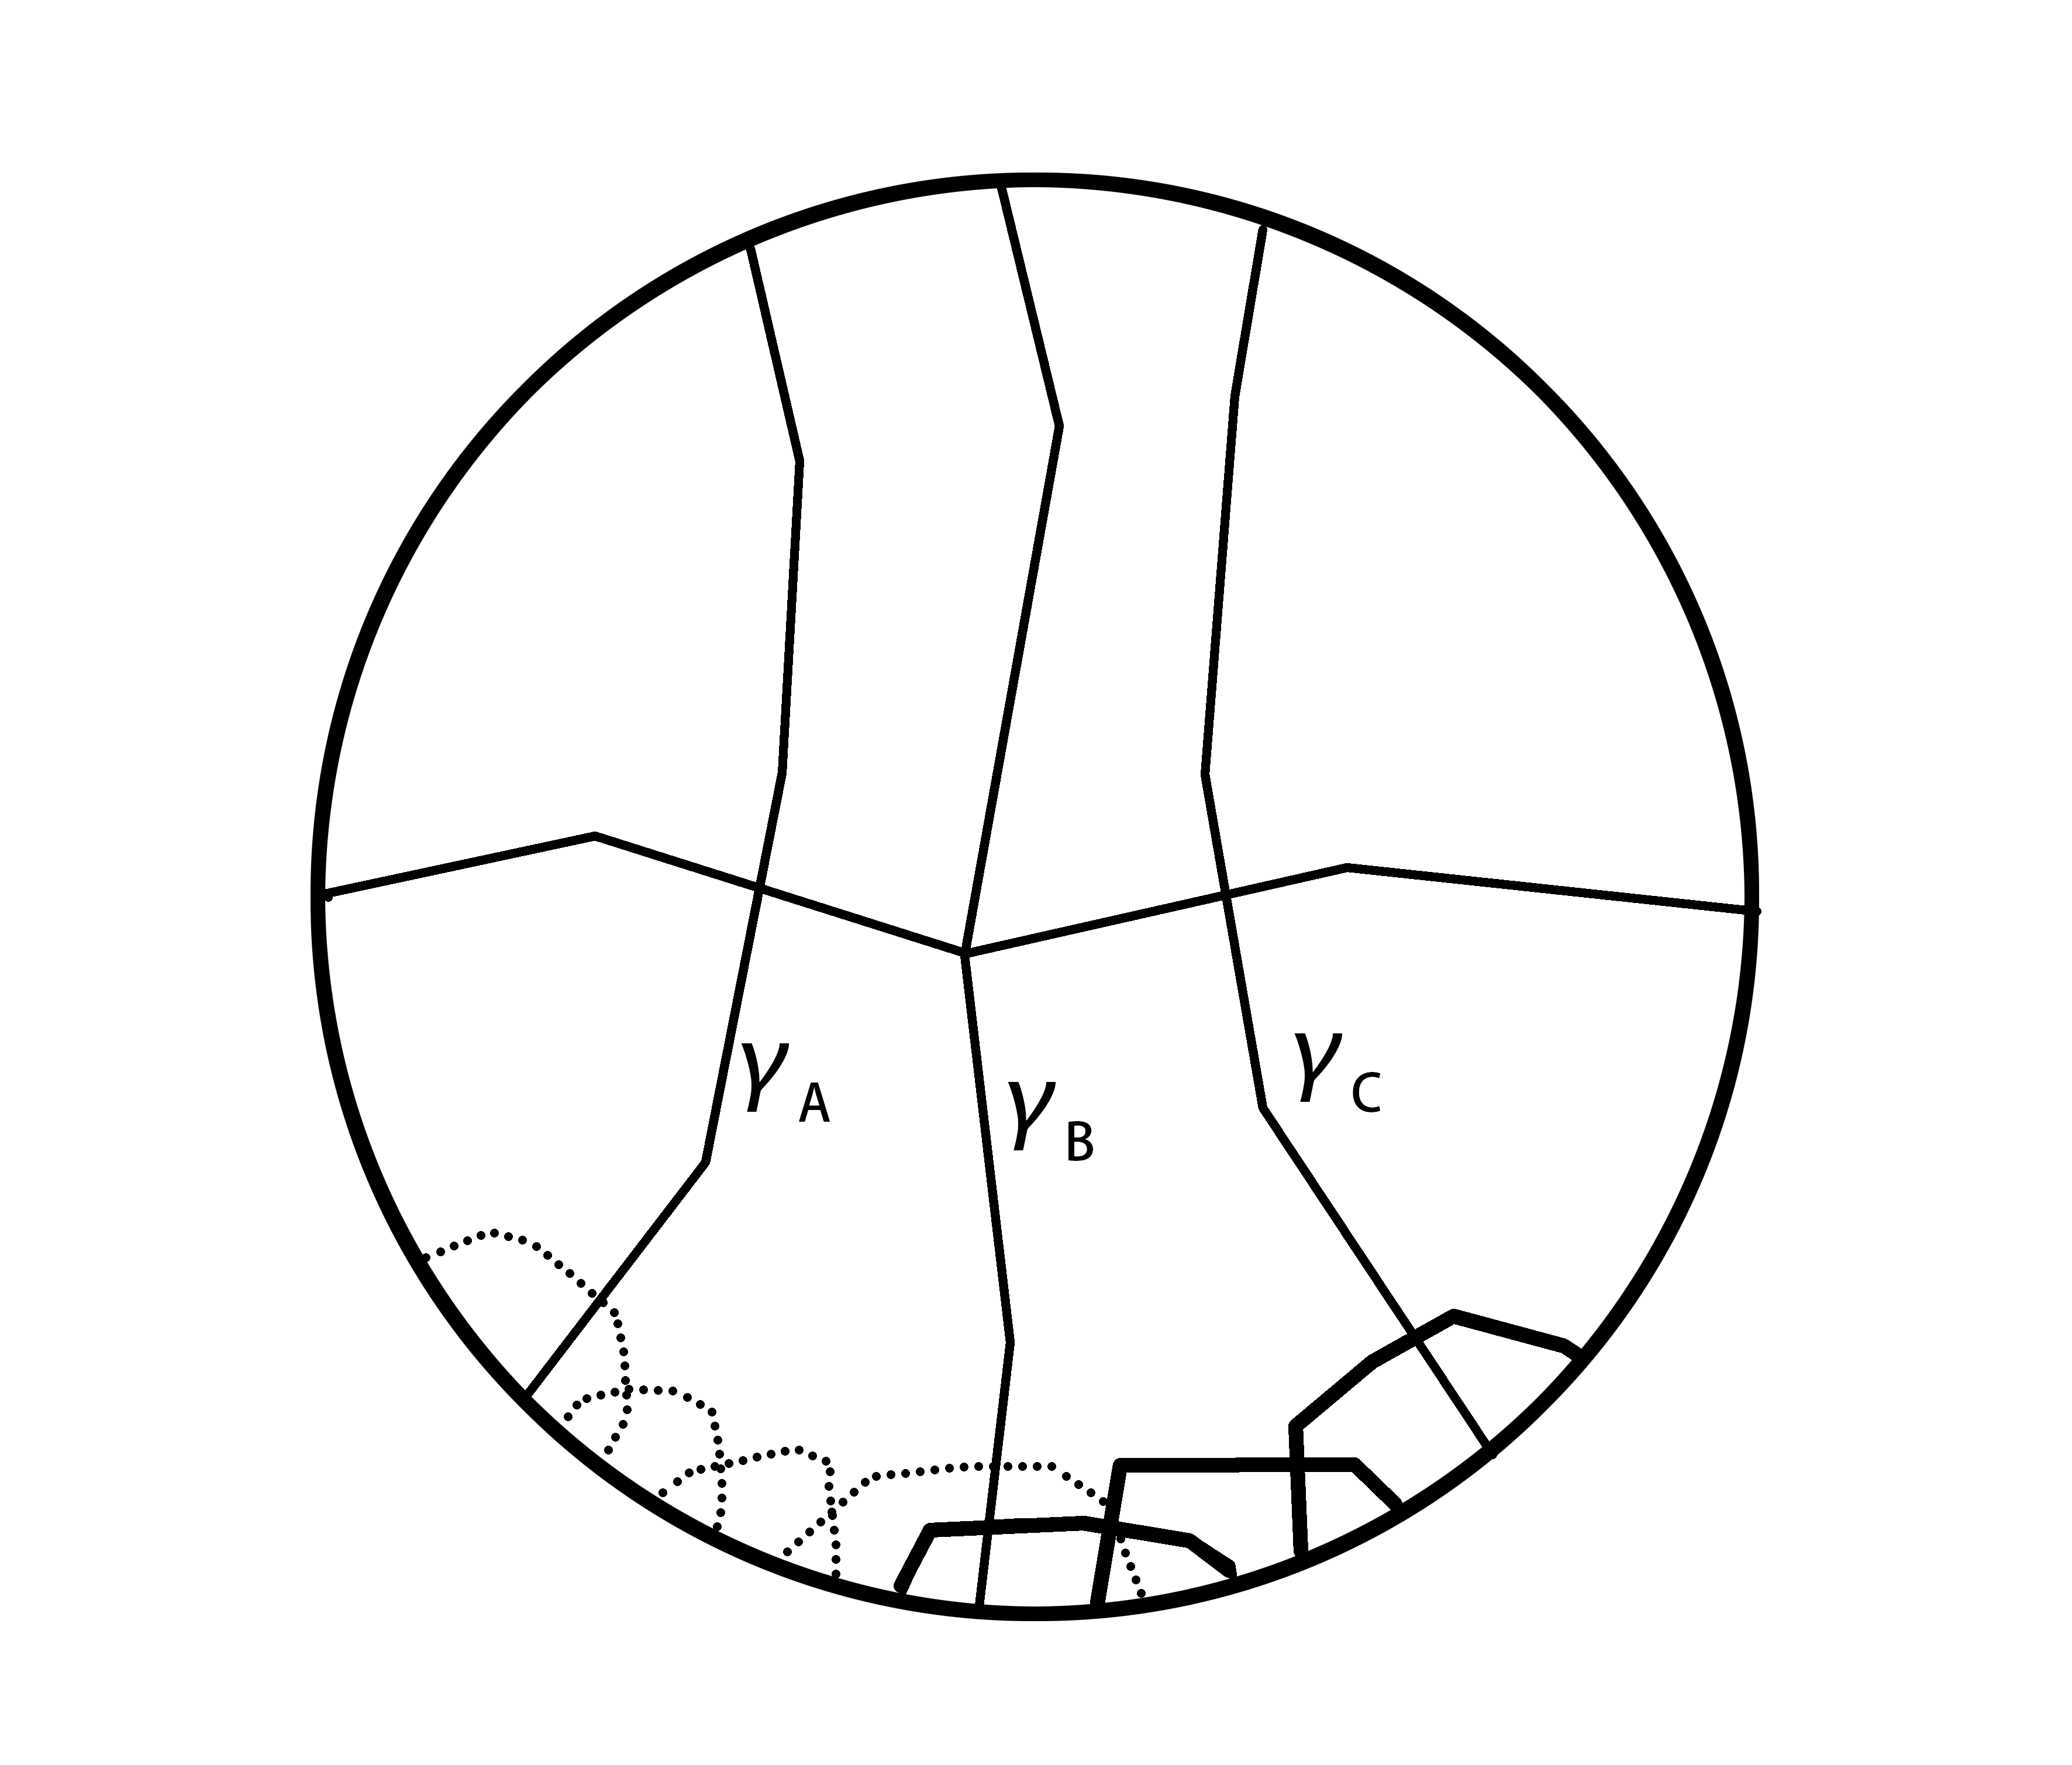
\includegraphics[scale=0.25]{geodesic_chain.png}
    \caption{Geodesic chains}
    \label{geodesic_chain}
\end{figure}
% 
% 
\begin{proof}
    Since $\mathbb{\mathbb{D}}$ is quasi-isometric to the hyperbolic plane $\mathbb{\mathbb{D}}_H$, every point \- $x \in (\gamma_A(+\infty), \gamma_B(+\infty))$ has a neighborhood $U_x$ such that for any two points $p, q\in U_x$, the geodesic connecting $p, q$ is disjoint from $\gamma$ and $\gamma_C$.  By compactness, we get a finite sequence of intervals $\{(a_n, b_n)\}_{0\le n \le N}$ such that their endpoints $a_0, a_1, b_0, a_2, b_1 \dots a_n, a_{n+1}, b_{n-1}, a_{n+1}, b_n \dots $ lie on $\partial \mathbb{\mathbb{D}}$ in counter-clockwise order, and $\gamma_A(+\infty) \in (a_0, b_0)$, and $\gamma_B(+\infty) \in (a_N, b_N)$.  For each $n$, take the geodesic connecting $a_n$ and $b_n$.  Then these geodesics make up a geodesic chain which we denote by $\Gamma_\alpha$.  Similarly, for the two endpoints $\gamma_B(+\infty)$ and $\gamma_C(+\infty)$, we get a geodesic chain $\Gamma_\beta$.  One can easily check that $\Gamma_\alpha$ and $\Gamma_\beta$ satisfy these conditions above.  In Figure \ref{geodesic_chain}, the dotted geodesics form a geodesic chain connecting $\gamma_A$ and $\gamma_B$, and the bold geodesics form a geodesic chain connecting $\gamma_B$ and $\gamma_C$.  
\end{proof}
% 
% 
\begin{Proposition} \label{middle-point-property}
    Let $g:\mathbb{R} \mapsto \mathbb{R}$ be an injective map.  If $g$ has the middle-point-preserving property, then $g$ is monotone.  
\end{Proposition}
\begin{proof}
    The proof is quite elementary.  Up to a homeomorphism of $\mathbb{R}$, we assume that $g(0)<g(1)$.  We now show that $g$ is strictly increasing.  Take two points $x, y \in \mathbb{R}$ and suppose that $x<y<0$.  Since $0$ is in the middle of $y$ and $1$, $g(0)$ is in the middle of $g(y)$ and $g(1)$.  Then it follows that $g(y) < g(0) < g(1)$. Since $y$ is in the middle of $x$ and $0$, it follows that $g(x) < g(y) < g(0)$. \par
    The other cases are similar.  We omit the  details.  
\end{proof}
% 
Any geodesic $\gamma$ divides the unit disk $\mathbb{D}$ into two parts.  Denote these two parts by $\mathbb{D}_\gamma^+$ and $\mathbb{D}_\gamma^-$.
\begin{proof}[Proof of Lemma \ref{order-preserving}]
    By Proposition \ref{middle-point-property}, we have only to prove that $f$ has the middle-point-preserving property.  We argue by contradiction.  Suppose that $f(A)$ is in the middle of $f(B)$ and $f(C)$. \par  %The geodesic $f(\gamma)$ divides $\mathbb{D}$ into two half-spaces and we denote them by $\mathbb{D}^+_{f(\gamma)}$ and $\mathbb{D}^-_{f(\gamma)}$.\par
    If $f(\gamma_A)$ lies totally on the half-space $\mathbb{D}^+_{f(\gamma)}$, then the geodesic chain $f(\Gamma_\alpha)$ also lies totally on $\mathbb{D}^+_{f(\gamma)}$ since it intersects $f(\gamma_A)$ and doesn't intersect $f(\gamma)$.  Similarly, since $f(\Gamma_\beta)$ intersects $f(\Gamma_\alpha)$ and doesn't intersect $f(\gamma)$, $f(\Gamma_\beta)$ lies totally on $\mathbb{D}^+_{f(\gamma)}$.  Take $P\in \gamma_B \cap \Gamma_\beta$ and $Q \in \gamma_C \cap \Gamma_\beta$.  Observe that $f(\gamma_A)$ divides $\mathbb{D}^+_{f(\gamma)}$ into three parts.  If two points $f(P)$ and $f(Q)$ lie on the same part, then either $f(\gamma_B)$ or $f(\gamma_C)$ intersects $f(\gamma_A)$ or $f(\gamma)$. If not, $f(\Gamma_\beta)$ intersects $f(\gamma_A)$ or $f(\gamma)$.  Anyway, we get a contradiction. \par 
    Otherwise, the two geodesics  $f(\gamma_B)$ and $f(\gamma_C)$ must lie on different sides of $f(\gamma_A)$.  Consider the geodesic chain $f(\Gamma_\beta)$.  It intersects both $f(\gamma_B)$ and $f(\gamma_C)$, and then it must intersect $f(\gamma_A)$.  Again, we get a contradiction.  
\end{proof}
% 
\begin{Corollary}
    For any geodesic $\gamma$, the restriction of $f$ to $\gamma:$ $f|_\gamma$ is a homeomorphism onto its image.  
\end{Corollary}
Since any segment or ray can be extended to a geodesic, we get the following corollary:
\begin{Corollary}
    The map $f$ maps every geodesic segment homeomorphically onto a geodesic segment and every ray homeomorphically onto a ray.  
\end{Corollary}
% 
\subsection{The map f is surjective}
\subsection*{} %I don't know why the next paragraph follows the title of the subsection “The map f is surjective” immediately if without this “\subsection*{}”
Fix any point $O\in D$.  The boundary $\partial \mathbb{D}$ can be naturally identified with all geodesic rays emanating from $O$.  Since $f$ maps every geodesic ray to a geodesic ray, it induces a map $\tilde{f}$ between $\partial \mathbb{D}$.  For any point $x \in \partial \mathbb{D}$, define $\tilde{f}(x)$ to be the endpoint of $f(\gamma_x)$, where $\gamma_x$ is the ray emanating from $O$ and tending to $x$.  Since any two geodesic rays emanating from the same point never share the same endpoint, $\tilde{f}$ is injective.  
% 
%Notice that $\tilde{f}$ depends on the choice of the basepoint $O$.  
% 
\begin{Lemma}
    The map $\tilde{f}$ is continuous.  
\end{Lemma}
\begin{proof}
    Fix a point $x_0 \in \partial \mathbb{D}$ and a small neighborhood $(a, b) \subset \partial \mathbb{D}$ of $x_0$.  Take a sequence of intervals $(a_n, b_n)$ satisfying the following conditions:
    \begin{enumerate}
        \item $x_0 = \mathop{\cap}_{n=0}^{+\infty}(a_n, b_n)$.  
        \item $(a, b)=(a_0, b_0)\supset (a_1, b_1) \supset.  .  .  \supset (a_n, b_n) \supset(a_{n+1}, b_{n+1}) \supset.  .  .  $
        \item $a_n \ne a_{n+1}$ and $b_n \ne b_{n+1}$ for each $n$.  
%       \item the endpoints $\{a_n, b_n\}$ of these intervals are all different.  
        \item The geodesic $\gamma_n$ connecting $a_n$ and $b_n$ is non-singular for each $n$.  \label{nonsingular-geodesic}
%       \item Both the two sequences $\{a_n\}$ and $\{b_n\}$ converge to $x_0$.  
    \end{enumerate}
    Only condition \eqref{nonsingular-geodesic} needs some explanation.  This is possible because of the following observation. Denote the ray connecting the two points $\{O,x_0\}$ by $\alpha$.  For each point $s\in \alpha$, take a geodesic $\gamma_s$ orthogonal to $\alpha$ at $s$.  Then we get a family of geodesics $\{\gamma_s\}_{s\in \alpha}$.  By Teichm\"uller's lemma, these geodesics are pairwise disjoint.  Since there are only countably many singular points, almost every geodesic in this family is non-singular.
%   Given any four different points $a, b, c, d \in \partial \mathbb{D}$ in counter-clockwise order.  Fix a homeomorphism $g:[a, b] \mapsto [c, d]$ with $g(a)=d$ and $g(b)=c$.  Consider the family of geodesics $\{\gamma_s\}_{s\in [a, b]}$ where $\gamma_s$ is the geodesic connecting $s$ and $g(s)$.  Obviously, these geodesics are pairwise disjoint.  Since there are only countably many singular points, almost every geodesic in this family is non-singular.  
%     
    We now show that $\tilde{f}(a_n)$ converges to $\tilde{f}(x_0)$.  Denote the geodesic connecting $a$ and $b$ by $\gamma$.  Since $f$ is a homeomorphism on $\gamma$, $\tilde{f}$ is order-preserving on $(a, b)$.  Denote the ray connecting $\{O, a_n\}$ by $\alpha_n$, and denote the geodesic connecting $\{a_k,b_k\}$ by $\gamma_k$.  Then for any $k<n$, $\gamma_k$ intersects $\alpha_n$.  Since $\gamma_k$ is non-singular, they intersect at a single point $p_{nk}$.  For any fixed $k$, $p_{nk}$ converges to $p_{k}$ where $p_k=\alpha \cap \gamma_k$.  Since $f$ is continuous on $\gamma_k$, the sequence $f(p_{nk})$ converges to  f($p_{k})$, which implies that $f(\alpha_n)$ converges to $f(\alpha)$ locally uniformly.  Therefore, $\tilde{f}(a_n)$ converges to $\tilde{f}(x_0)$.  For the same reason, $\tilde{f}(b_n)$ converges to $\tilde{f}(x_0)$.  In addition with the property that $\tilde{f}$ is order-preserving on $(a,b)$, we conclude $f$ is continuous at $x_0$.  
\end{proof}
% 
\begin{Corollary}
    The map $\tilde{f}$ is a homeomorphism.  
\end{Corollary}
\begin{proof}
    It is continuous, injective and proper.  
\end{proof}
% 
With the help of $\tilde{f}$, we can prove that $f$ is surjective.  
\begin{Corollary}
    The map $f$ is surjective.  
\end{Corollary}
\begin{proof}
    For any point $q \in \mathbb{D}$, take a geodesic ray $\alpha$ emanating from $f(O)$ and passing through $q$.  Denote the preimage $\tilde{f}^{-1}(\alpha(+\infty))$ by $x$.  The geodesic ray connecting $\{O, x\}$ is denoted by $\gamma_x$.  By the definition of $\tilde{f}$, $f(\gamma_x)$ is the geodesic ray connecting $\tilde{f}(x)$ and $f(O)$, which is exactly $\alpha$.  Thus, $\gamma_x$ is mapped homeomorphically onto $\alpha$ and $q$ must have a preimage.  
\end{proof}
% 
\subsection{The map f is a homeomorphism}
% 
\begin{Lemma}
    For any geodesic $\gamma$, if $p, q \in \mathbb{D}$ lie on the same side of $\gamma$, then $f(p)$ and $f(q)$ lie on the same side of $f(\gamma)$.  
\end{Lemma}
\begin{proof}
    Suppose that $p,q$ lie on the same side of $\gamma$.  Take two geodesic rays $\gamma_p, \gamma_q$ emanating from $p, q$ respectively.  Assume that they are both disjoint from $\gamma$ and their endpoints are away from the endpoints of $\gamma$.  This is possible by the following observation.  Fix a point $O \in \gamma$.  Take two geodesic rays $\alpha$ and $\beta$ emanating from $O$ and passing through $p$ and $q$ respectively.  Then the two subrays of $\alpha$ and $\beta$ starting from $p$ and $q$ respectively satisfy our requirements.  Take a geodesic chain $\Gamma_{pq}$ which is disjoint from $\gamma$ and connects the two rays $\gamma_p$ and $\gamma_q$.  Then the image of $\Gamma_{pq}$, $\gamma_p$ and $\gamma_q$ lie on the same side of $f(\gamma)$, and thus the lemma follows.  
\end{proof}
The above lemma implies that $f$ maps a half-space into a half-space.  In addition with surjectivity of $f$, we get the following corollary:
\begin{Corollary}\label{half-space-to-half-space}
    Given any geodesic $\gamma$, if there exists a point $p\in \mathbb{D}^+_\gamma$ such that $f(p)\in \mathbb{D}^+_{f(\gamma)}$, then  $f$ maps $\mathbb{D}^+_\gamma$ bijectively onto $\mathbb{D}^+_{f(\gamma)}$ and maps $\mathbb{D}^-_\gamma$ bijectively onto $\mathbb{D}^-_{f(\gamma)}$.  
\end{Corollary}
Obviously, the same conclusion also holds for the closed half-spaces $\mathbb{D}^+_\gamma \cup \gamma$ and $\mathbb{D}^-_\gamma \cup \gamma$
% 
\begin{figure}[h]
    \centering
    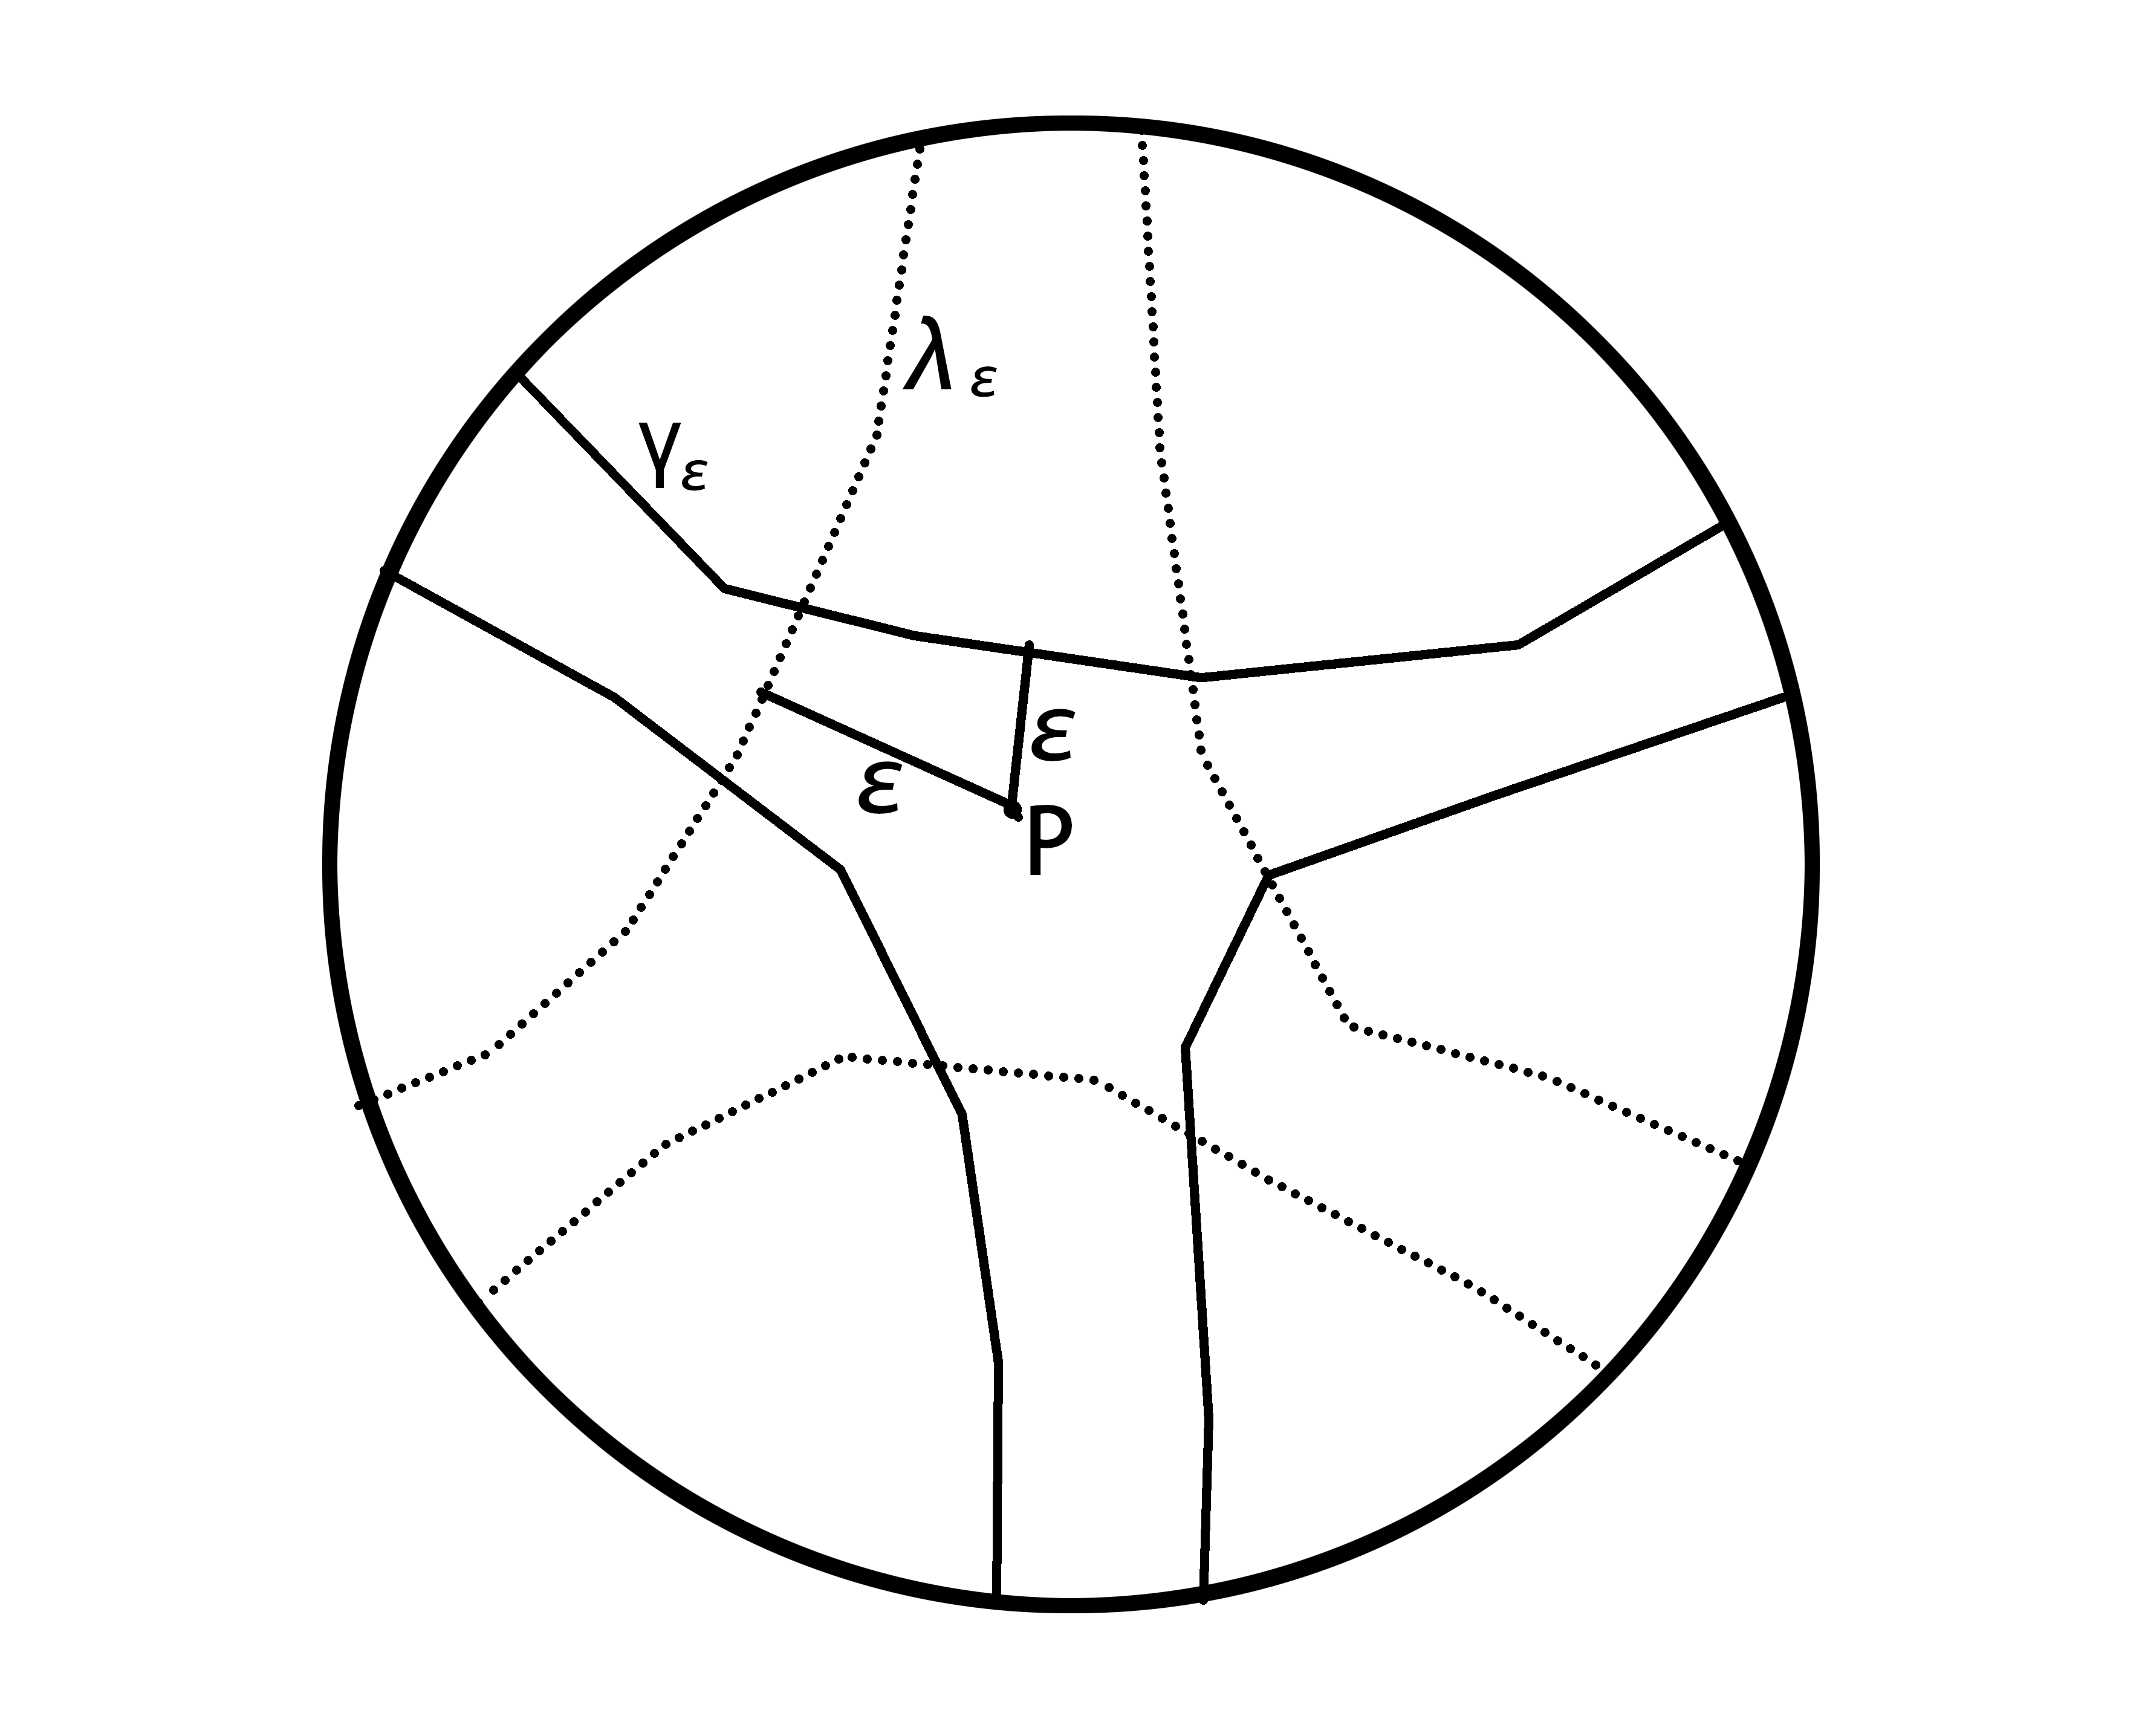
\includegraphics[scale=0.25]{small_neighborhood.png} 
    \caption{A small neighborhood bounded by horizontal and vertical geodesics}
    \label{small_neighborhood}
\end{figure}
% 
\begin{Lemma}
    The map $f$ is continuous.  
\end{Lemma}
\begin{proof}
For any point $p \in \mathbb{D}$, construct a sequence of neighborhoods $U_\epsilon$ of $p$ in the following way.  Take all vertical trajectories at the distance $\epsilon$ from $p$, and denote them by $\{\gamma^\epsilon_n\}_{1 \le n \le N}$ where $N-2$ is the order of $p$.  Take all horizontal trajectories at the distance $\epsilon$ from $p$ and denote them by $\{\lambda^\epsilon_n\}_{1 \le n \le N}$.  Then these horizontal and vertical trajectories bound a neighborhood $U_\epsilon$ of $p$.  It is easily seen $U_\epsilon=\{\cap \mathbb{D}^+_{\gamma^\epsilon_n}\} \cap  \{\cap \mathbb{D}^+_{\lambda^\epsilon_n}\}$ where $\mathbb{D}^+_{\gamma^\epsilon_n}$ or $\mathbb{D}^+_{\lambda^\epsilon_n}$ is the half-space containing $p$.  See Figure \ref{small_neighborhood}.  Take $\epsilon \to 0$, we get that $\mathop{\cap} \limits_{\epsilon \to 0} f(\overline{U_\epsilon}) = f(\mathop{\cap} \limits_{\epsilon \to 0} \overline{U_\epsilon})= f(p)$.  Then $f$ is continuous at $p$.  Since $p$ is arbitrary, $f$ is a continuous bijection. 
\end{proof}
\begin{Corollary}
    The map $f$ is a homeomorphism.
\end{Corollary}
% 
% 
\frac{aab}{bb}
\frac{ddddddd}{bbbbb}
% 
\subsection{The map f is affine}
\subsection*{} 
Theorem \ref{main_theorem} now follows from a variation of the classical Pappus's Theorem.  There's a detailed introduction to this theorem and its generalizations in \cite{LiWangFundamental2016}.  For completeness, we include a brief proof here of what we need.  
\begin{Lemma}
    Given a triangle  $\triangle OP_3Q_3$ on the Euclidean plane, suppose that there are two pairs of points $\{P_1, P_2\}$, and that $\{Q_1, Q_2\}$ on $OP_3$ and $OQ_3$ respectively, as shown in Figure \ref{colinear}.  Fix the two lines $P_1Q_1$ and $P_2Q_2$.  Move $Q_3$ along the segment $Q_3P_3$ towards $P_3$.  During this process, suppose that  $P_1Q_2, P_2Q_1$ intersect at M and $P_2Q_3, P_3Q_2$ intersect at N.  Then $P_1Q_1, P_2Q_2$ and $P_3Q_3$ are parallel if and only if the three points $\{O, M, N\}$ are always colinear when we move $Q_3$ towards $P_3$.  
\end{Lemma}
\begin{figure}[h]
    \centering
    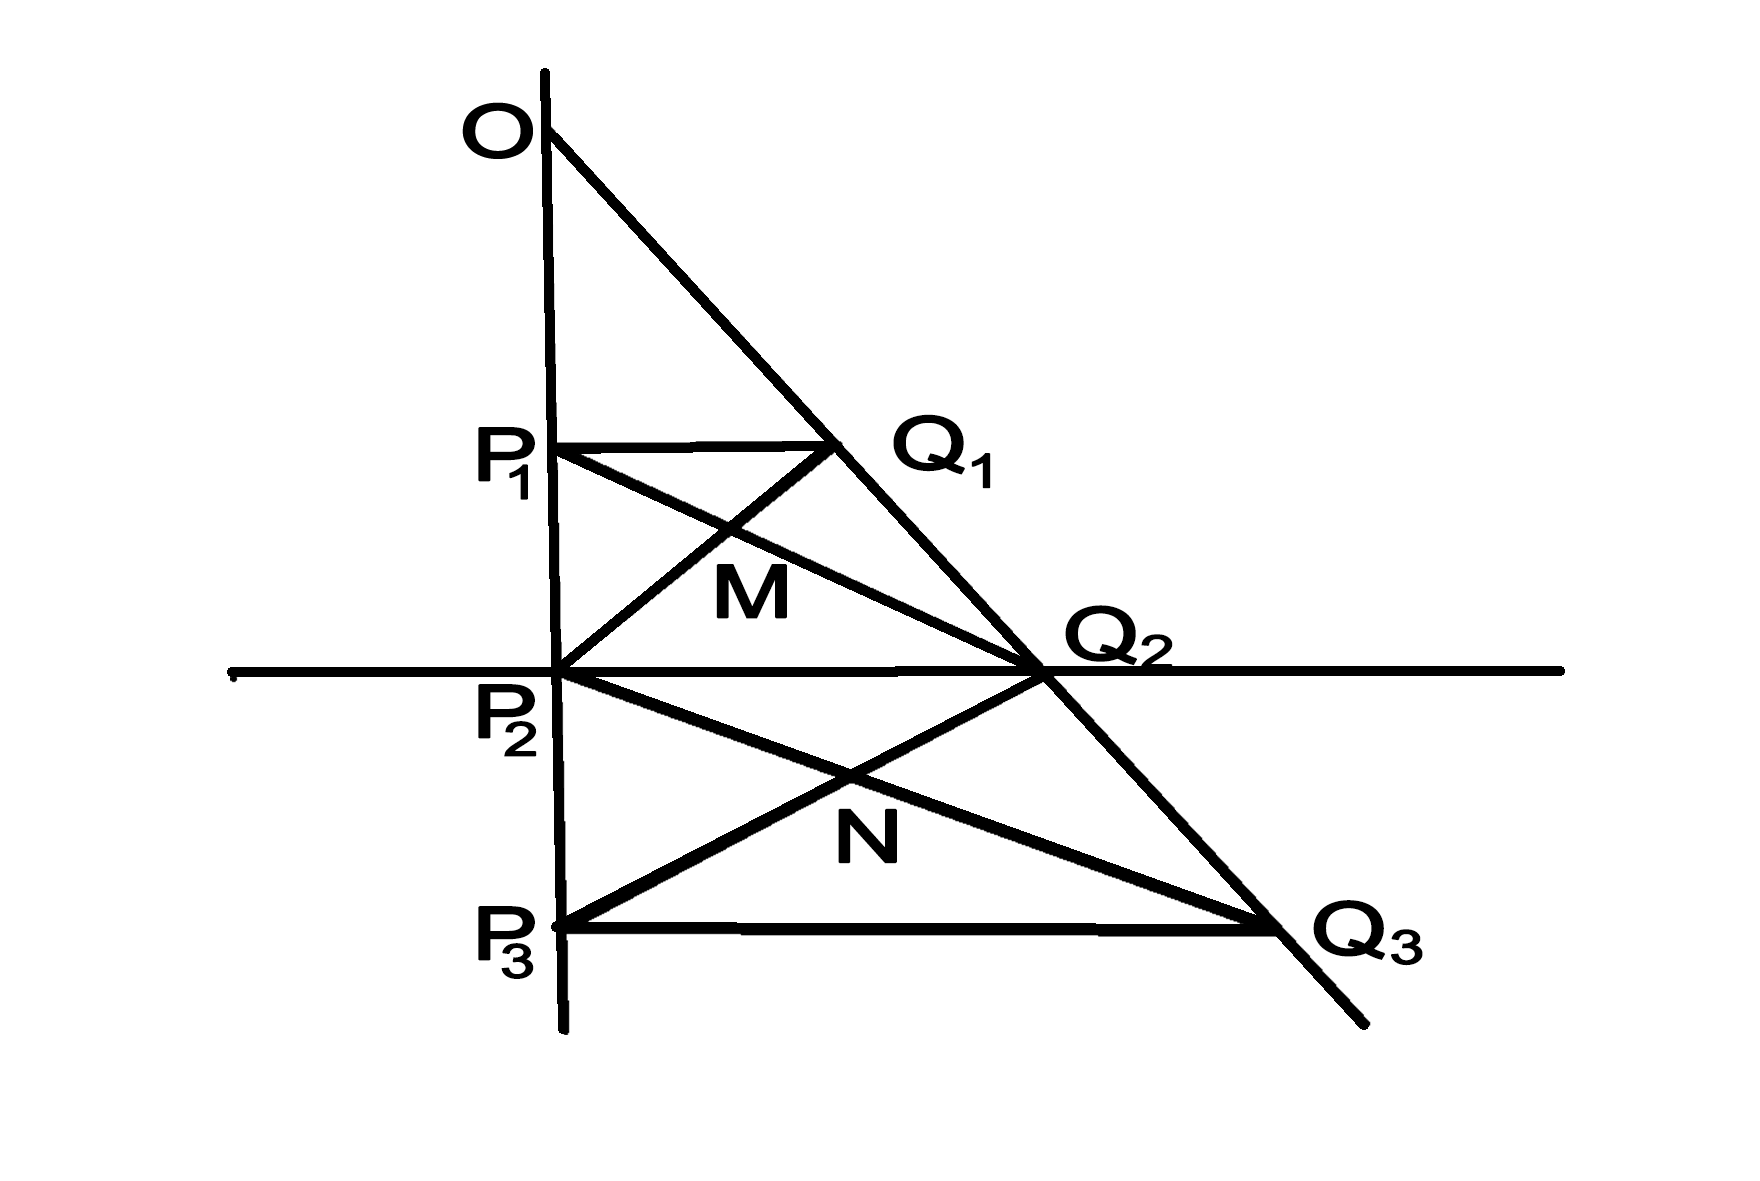
\includegraphics[scale=0.5]{colinear.png}
    \caption{Pappus's Theorem}
    \label{colinear}
\end{figure}
\begin{proof}
    Up to an affine map of $\mathbb{R}^2$, we can assume that $P_2=(0, 0), O=(0, 1), P_1=(0, a), P_3=(0, b)$ and $Q_2=(c, 0)$.  Denote the slopes of $P_1Q_1$ and $P_3Q_3$ by $k_1$ and $k_2$ respectively.  The coordinate of a point $Z$ is represented by $(x_Z, y_Z)$.  By a direct computation, we get the coordinates of $M$ and $N$.  
    \begin{equation*}  
    \left\{
    \begin{aligned}
    &(x_M, y_M)=(\frac{(1-a)ac}{k_1c+2a-a^2}, \frac{k_1ac+a^2}{k_1c+2a-a^2})\\
    &(x_N, y_N)=(\frac{(1-b)bc}{k_2c+2b-b^2}, \frac{k_2bc+b^2}{k_2c+2b-b^2})\\
    \end{aligned}
    \right.  
    \end{equation*}  
    An elementary computation shows that $OM \parallelsum ON$ for any $c$ if and only if $k_1=k_2=0$.  
    The other direction is obvious.  
\end{proof}
\begin{proof}[Proof of Theorem \ref{main_theorem}]
    The above lemma implies that $f$ maps parallel geodesics to parallel geodesics.  Fix a square small $Q\subset \mathbb{D}$.  The central point of $Q$ is denoted by $O$ and the horizontal and vertical geodesics through $O$ are denoted by $\alpha$ and $\beta$ respectively. Up to an affine map, we may assume that $f$ maps $Q$ homeomorphically onto itself and fixes the four vertexes of $Q$.  Then it necessarily fixes the central point $O$, and thus leaves $\alpha$ and $\beta$ invariant.  Observe that $\alpha$ and $\beta$ divide $Q$ into four squares. We can see that each $\frac{1}{4}$ subsquare of $Q$ is invariant under $f$.  By an inductive argument, we see that $f$ is the identity map on $Q$.  We complete the proof of Theorem \ref{main_theorem}.  
\end{proof}
\nocite{*}
\printbibliography
\end{document}
